\chapter{Incentives and Truthfulness}
\label{cha:incentives_and_truthfulness}


\section{Motivating Example: Incentives to Report Multiple Donors}
\label{sec:incentives}

Let's begin by defining the incentives of each patient-donor group. Naturally, the primary goal of each group is to obtain a compatible kidney for the associated patient. Secondarily, each group aims to minimize its loss, that is, the number of proxy kidneys it gives up in exchange for a compatible kidney. This leads to the following ranking of possible outcomes for each group, ordered from most to least desirable:

\begin{enumerate}
\item Receive one compatible kidney and lose 0 proxy kidneys.
\item Receive one compatible kidney and lose 1 proxy kidney.
\item Receive one compatible kidney and lose 2 proxy kidneys.
\item Receive no compatible kidney and lose 0 proxy kidneys.
\end{enumerate}

Note that we do not consider a case where a group receives no compatible kidney but still loses a proxy kidney. If that was the outcome for some group, the groups would simply refuse to participate. Furthermore, if a group chooses to participate as an alternative-donors group, the third outcome is not taken as an option for this group.

It is not immediately obvious whether participating in the \textit{multiple-donors} program provides any advantage for a patient-donor group compared to participating in the \textit{alternative-donors} program. The example in \autoref{fig:incentive_motivation_example2} clarifies this question. In \textbf{(a)}, we see an example graph where patient $p_1$ has two proxy donors: $d_1^1$ and $d_1^2$. The graph includes two overlapping cycles: one of length two that includes $p_1$, and another of length three that does not. In the solution, only one of these cycles can be selected.

If patient $p_1$ chooses to report their donors as alternative donors, $d_1^1 \oplus d_1^2$, then the system (which maximizes the number of transplants) will select the longer cycle (the orange one in \textbf{(b)}), resulting in $p_1$ not receiving a compatible kidney. On the other hand, if $p_1$ is willing to use both proxy donors, then (as shown in \textbf{(c)}) the system will select the cycle of length two that includes $p_1$ and the chain initiated by $d_1^2$, also of length two, saving a total of four patients.

This scenario is not far removed from real life. Imagine that $p_1$ is a child in need of a kidney transplant, and $d_1^1$ and $d_1^2$ are the child’s parents—both incompatible with the child but willing to do anything to help. The \textit{multiple-donors} model opens new possibilities for such groups in these situations.

\begin{figure}
    \centering
    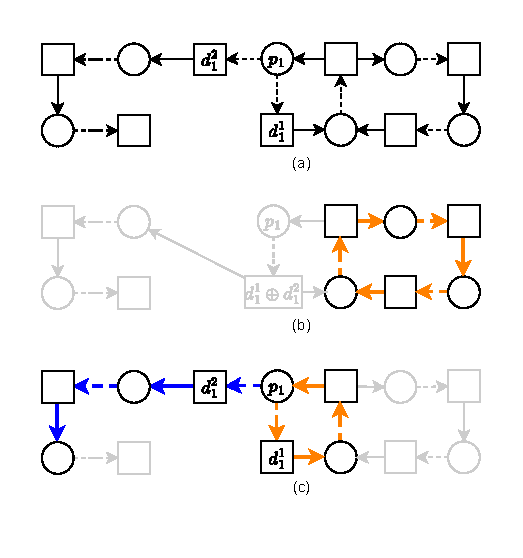
\includegraphics{data/incentive_motivation_example2.pdf}
    \caption[An example showing the benefit of reporting two proxy donors in multiple-donors model]{\textbf{(a)} shows an example of a graph containing two overlapping cycles, where the left cycle contains patient $p_1$ who has two proxy donors: $d_1^1$ and $d_1^2$. In \textbf{(b)} patient $p_1$ reports his donors as alternative donors $d_1^1 \oplus d_1^2$ and in result don't receive a compatible kidney. \textbf{(c)} shows that by reporting two proxy donors in the multiple-donors model, patient $p_1$ receives a compatible kidney in exchange for two proxy kidneys.}
    \label{fig:incentive_motivation_example2}
\end{figure}

\section{Truthfulness in the Multiple-Donors Model}
Unfortunately, the \textit{multiple-donors} model, together with the incentives discussed in \autoref{sec:incentives}, forces patients to act strategically. The question every patient will ask themselves is whether they should report all donors. If they report two donors, they risk both donors losing their kidneys, while in reality, reporting only one might be sufficient for the patient to receive a kidney. We consider two types of truthfulness.

\begin{definition}[Truthfulness]
We say a kidney exchange mechanism is \emph{truthful} if, for each group, donating more proxy kidneys implies receiving strictly more compatible kidneys. In other words, to satisfy truthfulness, the system should take two proxy kidneys from a group if and only if taking one of the proxy kidneys would not result in the patient of the group receiving a compatible kidney.
\end{definition}

\begin{definition}[Weak Truthfulness]
We say a kidney exchange mechanism is \emph{weakly truthful} if, for each group, reporting more proxy donors implies receiving at least as many compatible kidneys. That is, if a group reports only one proxy donor and receives a compatible kidney, then the same group would also receive a compatible kidney if it reported more proxy donors.
\end{definition}

Of course, truthfulness implies weak truthfulness, but not vice versa.

\subsection{Truthfulness}
\begin{lemma}
    \label{lemma:social_walfare_not_strongly_truthful}
    Social-welfare maximizing multiple donor model is not truthful.
    \begin{proof}
        Let there be an algorithm $A$ solving \textit{social-welfare maximizing multiple donors} problem and consider the example graph from \autoref{fig:multiple_model_example}. In the example, if patient $p_2$ reports both of his proxies; $d_2^1$ and $d_2^2$, $A$ assigns him a compatible kidney from $d_1$ in exchange for two proxy donors. On the other hand, if patient $p_1$ decides to hide donor $d_2^2$, $A$ assigns him a kidney from $d_1$ in exchange for only one proxy kidney $d_2^1$.
    \end{proof}
\end{lemma}


Moreover, knowing the structure of the graph in the social-welfare maximizing problem gives player an advantage, this is perfectly depicted in \autoref{fig:prisoners_dilemma} which shows two patients being in the Prisoner's Dilemma situation. In the example, two patients $p_1$ and $p_2$ have two proxy donors; $d_1^2$, $d_2^2$ and $d_2^1$, $d_2^2$ respectively. Both patients are in the same cycle of length 3 which overlaps with a larger one of length 4. If both decide to only report one of their donors (as shown in \textbf{(b)}), the larger cycle is selected in the solution, and both patients end up without compatible kidney. If both decide to report all of theirs donors (see \textbf{(c)}), the smaller cycle is selected together with two chains, each of length 2, summing up to 7 patients saved. In this case both patients receive a compatible kidney but at the same time both lose two of theirs proxy donors. If patient $p_1$ knows the structure of the graph and knows that $p_2$ will report two of his donors, then, he can decide to hide donor $d_1^2$ (see \textbf{(d)}). In that case, small cycle is selected together with one chain on length 2 initiated by $d_2^2$ summing up to total 5 patients saved. Notably, patient $p_1$ received a compatible kidney and spent only one of his donors, while, $p_2$ spent two of his proxies.


\begin{figure}
    \centering
    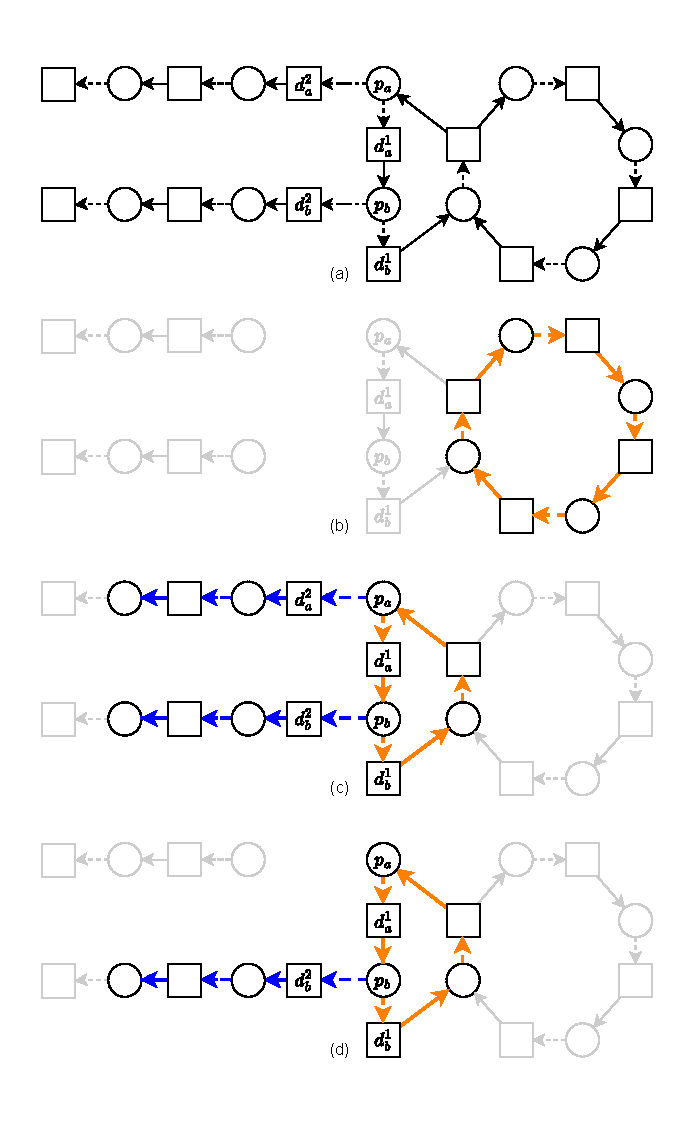
\includegraphics{data/prisoners_dilemma.pdf}
    \caption[Prisoner's dilemma in multiple-donors model]{\textbf{(a)} illustrates a graph where patients $p_1$ and $p_2$ are in \textit{Prisoner's Dilemma} situation. \textbf{(b)} shows that if both $p_1$ and $p_2$ decide not to report $d_1^2$ and $d_2^2$ respectively, they both don't receive compatible kidney in the final solution. In \textbf{(c)}, both patients reported both of theirs donors, they both receive compatible kidney but also they both spent two kidneys of their proxy donors. In \textbf{(d)}, patient $p_2$ reported both of his proxy donors, patient $p_1$ reported only $d_1^1$. In this case, $p_1$ gets a compatible kidney and spends only one proxy kidney. Patient $p_2$ gets a compatible kidney as well but spends two proxy kidneys. The symmetric case occurs when $p_1$ reports two proxy donors and $p_2$ reports only one of his proxies.}
    \label{fig:prisoners_dilemma}
\end{figure}

\subsection{Weak Truthfulness}
When it comes to weak truthfulness, not every algorithm that solves the social-welfare maximizing multiple donor problem possesses this property. This is demonstrated in the following lemma.

\begin{lemma}
\label{lemma:weak_truthfulness_false}
    Not every algorithm solving the social-welfare maximizing multiple donors problem has weak truthfulness property.
    \begin{proof}
        Consider, for example, the simple graph illustrated in \autoref{fig:weak_truthfulness}, and let us examine an algorithm $A$ that solves the model without a consistent tie-breaking rule. That is, if there are multiple optimal solutions, the algorithm deterministically\footnote{Here, \textit{deterministically} means that given the same graph twice, the algorithm will always return the same solution for both instances.} returns one of them arbitrarily.
    
        In this example, patient-donor groups form two overlapping cycles, each of length two. The algorithm can select only one of these cycles in its solution. Suppose $A$ selects the left cycle, as shown in \textbf{(a)}, thereby assigning a compatible kidney to patient $p_1$. In \textbf{(b)}, the same patient $p_1$ reports an additional proxy donor $d_1^2$, who is not compatible with any patient in the graph. Although this addition does not affect the number of patients that can be saved, it changes the structure of the graph and may cause $A$ to select the right cycle instead, which does not include $p_1$.
    \end{proof}
\end{lemma}

The proof of the previous lemma shows that inconsistent tie-breaking is the reason an algorithm may fail to be weakly truthful. In the next lemma, we show that an algorithm with an arbitrary consistent tie-breaking rule is weakly truthful. Before  we do that, let's define what consistent tie-breaking even means.

\begin{definition}[Consistent tie-breaking rule]
\label{consistent_tie_breaking_rule}
    Given the set $S_k$ of all solutions that achieve the same score $k$ (i.e., the same number of patients saved), a consistent tie-breaking rule imposes a strict, arbitrary ordering over $S_k$ that is independent of the reports provided by patient-donors groups. For any input graph $G$ where the maximum number of patients that can be saved is $k$, the rule selects the highest-ranked valid solution from $S_k$ according to this fixed ordering.
\end{definition}

A particularly appealing consistent tie-breaking rule is based on assigning priorities among the patients, similar to how waiting lists for kidneys from deceased donors are handled. In such lists, patients are ranked according to a fixed priority score that reflects medical urgency, ethical considerations, or logistical factors. When a kidney becomes available, it is allocated to the highest-priority patient among those compatible with the organ. Translating this idea to our mechanism design setting, we can impose a consistent tie-breaking rule by predefining a strict priority ordering over the agents. When multiple allocations yield the same utility, the tie is broken in favor of the allocation that benefits the agent with the highest priority.

\begin{lemma}
    An algorithm with a consistent tie-breaking rule solving the social-welfare maximizing multiple donors model is weakly truthful.
    \begin{proof}
    Let $A$ be an algorithm with a consistent tie-breaking rule (as defined in \autoref{consistent_tie_breaking_rule}) that solves the social-welfare maximizing multiple donors problem, and consider an arbitrary graph $G$ in which patient $p_1$ reports one proxy donor $d_1^1$. Assume that, given $G$, $A$ returns a solution $s$ in which $p_1$ receives a compatible kidney.
    
    Now, construct a graph $G'$ with the same structure as $G$, but where $p_1$ has an additional proxy donor $d_1^2$. If this addition increases the maximum number of patients saved, it implies that $d_1^2$ is used, and therefore $p_1$ still receives a compatible kidney.
    
    If the addition of $d_1^2$ does not increase the number of patients saved (i.e., the optimal value remains the same), then the solution returned by $A$ in $G'$ must still belong to the set $S_k$ of solutions that save $k$ patients. Since $A$ uses a consistent tie-breaking rule and the ordering over $S_k$ is fixed independently of the reports, the algorithm will either:
    \begin{enumerate}
        \item Return the same solution $s$ as before, in which $p_1$ receives a compatible kidney; or
        \item Return a different solution $s' \in S_k$ that is ranked higher than $s$ according to the consistent ordering. This change can only occur if $d_1^2$ is used, which again implies that $p_1$ receives a compatible kidney.
    \end{enumerate}
    \end{proof}
\end{lemma}



\begin{figure}
    \centering
    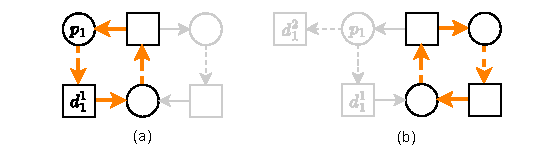
\includegraphics{data/weak_truthfulness.pdf}
    \caption[An example output of an algorithm without a consistent tie-breaking strategy.]{Example outputs from an algorithm solving the social-welfare-maximizing multiple donors model without a consistent tie-breaking strategy. In \textbf{(a)}, the algorithm selects the left cycle of length 2, assigning $p_1$ a compatible kidney. In \textbf{(b)}, patient $p_1$ reports an additional 'dangling' donor $d_1^2$. This time, the algorithm selects the right cycle of length 2, which is equally compelling, resulting in patient $p_1$ not being matched to a compatible kidney.}
    \label{fig:weak_truthfulness}
\end{figure}


\section{Achieving Truthfulness via Randomized Mechanisms}

As discussed earlier, no deterministic algorithm can simultaneously guarantee both truthfulness and maximum social welfare in our setting. The core issue is that if a patient can obtain a kidney by reporting only one donor, they have no incentive to report both; the additional donor does not improve their utility. This misalignment can be mitigated by introducing randomness into the mechanism.

The key idea is to shift the notion of utility: instead of a binary outcome (receiving a kidney or not), we consider the probability of receiving a kidney as the utility. This enables a simple incentive structure: the more donors a patient truthfully reports, the higher their probability of being matched.

Suppose we have an algorithm $A$ that solves the maximum social welfare problem, which is not truthful but weakly truthful. We can construct a randomized algorithm $R$ that is truthful, using the following procedure:

\begin{enumerate}
    \item Run the original algorithm $A$ and obtain its output.
    \item Let the output include $n$ patients, and suppose these patients have collectively reported $m$ donors. Let $\epsilon > 0$ be a small constant.
    \item Return the output of $A$ with probability $1 - (2n - m)\epsilon$; otherwise (with probability $(2n - m)\epsilon$), return an empty allocation.
\end{enumerate}

The expected performance of $R$ satisfies:
\[
\lim_{\epsilon \to 0^+} \frac{\mathbb{E}[R]}{O} = 1 - (2n - m)\epsilon = 1,
\]
implying that the randomized algorithm $R$ achieves nearly the same performance as $O$ when $\epsilon$ is small.

The underlying intuition is straightforward: the key factor for incentive alignment is whether a patient receives a kidney. In the randomized mechanism, patients are incentivized to report as many valid donors as possible. The more donors they report, the smaller the quantity $(2n - m)$ becomes, thereby reducing the probability that the output is discarded and increasing their expected utility.

\begin{lemma}
Let $A$ be an algorithm that is weakly truthful. Then the randomized mechanism $R$ constructed as described is truthful.
\end{lemma}

\begin{proof}
(Proof sketch) To show that the randomized mechanism $R$ is truthful, consider a report profile $s$ in which all patients report truthfully, and let patient $i$ report both of their available donors. Let $s_{-i}$ denote a modified report where patient $i$ misreports by reporting only one of the two donors.

Suppose first that, under $s_{-i}$, patient $i$ receives a kidney in the output of algorithm $A$. Since $A$ is weakly truthful, patient $i$ would also receive a kidney under $s$. Therefore, in the randomized mechanism $R$, the probability that patient $i$ receives a kidney under $s$ is strictly higher than under $s_{-i}$, since the value $(2n - m)$ is smaller when both donors are reported. That is, $R(s)$ has a higher expected utility than $R(s_{-i})$.

Now suppose that under $s_{-i}$, patient $i$ does not receive a kidney in $A$. In that case, reporting both donors cannot result in a worse outcome under $R$, and may result in a better one. In both scenarios, truthful reporting yields weakly higher expected utility.

Thus, for every patient, reporting all available donors is a dominant strategy in the randomized mechanism $R$, and therefore $R$ is truthful.
\end{proof}

%%% Local Variables:
%%% mode: latex
%%% TeX-master: "../ClassicThesis"
%%% ispell-dictionary: "british" ***
%%% fill-column: 76 ***
%%% End:
